% /*@@
%   @file      documentation.tex
%   @date      16 April 2002
%   @author    Denis Pollney
%   @desc 
%              Cartoon2D user/maintainer guide.
%   @enddesc 
%   @version $Header$      
% @@*/


\documentclass{article}

% Use the Cactus ThornGuide style file
% (Automatically used from Cactus distribution, if you have a 
%  thorn without the Cactus Flesh download this from the Cactus
%  homepage at www.cactuscode.org)
\usepackage{../../../../../doc/latex/cactus}

\newlength{\tableWidth} \newlength{\maxVarWidth} \newlength{\paraWidth} \newlength{\descWidth} \begin{document}

\title{Using Cartoon2D}
\author{Denis Pollney}
\date{$ $Date$ $}

\maketitle

% Do not delete next line
% START CACTUS THORNGUIDE

\begin{abstract}
  The \texttt{Cartoon2D} thorn allows fully 3D codes to be used
  to model axisymmetric systems, by considering a 3D evolution which
  is only one plane thick and applying a rotational tensor
  transformation to the flat faces of the plane as a boundary
  condition. This allows 3D codes to be tested efficiently on 2D
  problems, as well as providing a means of carrying out axisymmetric
  evolutions in cartesian coordinates without problems at the axis.
\end{abstract}

\section{Background}

The \texttt{Cartoon2D} thorn is the implementation of an idea first
presented in \cite{Alcubierre-etal-2001}. The principle is to use a
3-dimensional Cartesian $(x,y,z)$ coordinate grid which covers the
$y=0$ plane, but is only one finite difference molecule in width in
the $y$-direction. The field variables in the $y=0$ plane can be
updated using standard 3D $(x,y,z)$ coordinate finite differencing,
with off-plane derivatives calculated by performing appropriate
rotations of field variables using the axisymmetic assumption.
This technique has the advantage of removing a number of the axis
problems normally associated with axisymmetric codes.

The `cartoon' method was first implemented in Cactus3 by Steve Brandt
and Bernd Br\"ugmann, and was translated to Cactus4 by Sai
Iyer. Details of the method can be found in
\cite{Alcubierre-etal-2001}. This document provides a practical guide
to using the thorn as it is currently implemented.

\section{Basic usage}

Only a small number of parameters need to be set to use
\texttt{Cartoon2D}.

\begin{description}

  \item[\texttt{cartoon\_active}] A flag which determines whether or
  not the cartoon boundary condition should be applied. This should be
  set to ``yes'' to use \texttt{Cartoon2D}, otherwise the evolution
  will be assumed to be standard 3D.

  \item[\texttt{order}] Determines the order of interpolations to be
  carried out. This will determine the number of ghost zones that you
  need to specify in the $y$-direction.

  \item[\texttt{allow\_grid\_resize}] When this flag is set to
  ``yes'', \texttt{Cartoon2D} is allowed to modify the grid sizes
  specified in the parameter file so that a cartoon-compatible grid is
  used. See below.

  \item[\texttt{verbose}] Causes \texttt{Cartoon2D} to print a lot of
  messages.

%
% FIXME: The param.ccl file also mentions a stencil parameter, which
% seems not to be used in the code.
%

\end{description}

For example, the following is a section of a parameter file which sets
up a cartoon-style grid in bitant mode.
\begin{verbatim}

activethorns                            = "cartoon2d cartgrid3d pugh"

cartoon2d::cartoon_active               = "yes"
cartoon2d::order                        = 3
cartoon2d::allow_grid_resize            = "yes"

grid::type                              = "byspacing"
grid::domain                            = "bitant"
grid::bitant_plane                      = "xy"
grid::dxyz                              = 0.2

driver::global_nx                       = 16
driver::global_ny                       = 3
driver::global_nz                       = 16

driver::ghost_size_x                    = 2
driver::ghost_size_y                    = 1
driver::ghost_size_z                    = 2

driver::processor_topology              = "manual"
driver::processor_topology_3d_x         = 1
driver::processor_topology_3d_y         = 1
driver::processor_topology_3d_z         = 2

grid::avoid_originy                     = "no"

\end{verbatim}
The following features are worth noting:
\begin{itemize}

  \item The \texttt{order} parameter specifies that 3rd order
  interpolation is to be used. This requires that only one ghost zone
  is required in the y direction (\texttt{ghost\_size\_y}). If 4th
  order interpolation was specified, then two ghost zones would be
  required.

  \item The \texttt{allow\_grid\_resize} flag has been set, allowing
  \texttt{Cartoon2D} to modify the grid appropriately so that, for
  instance, it only extends a given number of ghost zones beyond the
  $z$-axis.

  \item The bitant plane should always be ``\texttt{xy}'', which means
  that only the positive $z$-axis is evolved and a reflection boundary
  is imposed along $z=0$.

  \item Though not necessary, it is often helpful to specify the
  processor topology explicitly to ensure that that only one processor
  is allocated to the $y$ direction, and that the processors in the
  $x$ and $z$ directions reflect the relative lengths of these axes
  (though in this example it doesn't matter which of these axes gets
  two processors).

  \item The \texttt{avoid\_originy} parameter needs to be turned off
    so that the cartoon plane corresponds to $y=0$.

\end{itemize}
Also, it is important to keep in mind that other thorns may also
require their own parameters to be set in order to interact
appropriately with \texttt{Cartoon2D}. For instance, see Section
\ref{sec:interaction}. Examples of working parameter files can be
found in the \texttt{Cartoon2D/test/} directory.

\begin{figure}
  \centering
  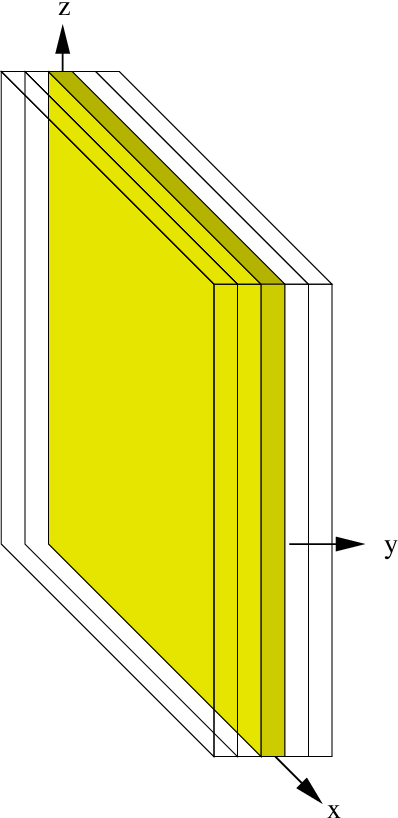
\includegraphics[angle=0,height=8cm]{/home/runner/work/einsteintoolkit/einsteintoolkit/arrangements/CactusNumerical/Cartoon2D/doc/cartoon_plane}
  \caption{The cartoon plane layout. The symmetry axis is the
    $z$-axis, with grid functions defined on the $y=0$ plane, in this
    example with two ghost zones.}
\end{figure}

\section{Automatic grid re-sizing}
\label{sec:regrid}

The \texttt{Cartoon2D} thorn has some non-standard requirements of the
grid which is normally set up by the \texttt{grid} implementation (for
instance, by \texttt{CartGrid3D}). In particular,

\begin{itemize}

  \item the grid in the $y$ direction should be exactly one plane in
    width, plus twice the number of $y$ ghost zones.

  \item the grid in the $x$ direction only needs to extend to the
    $z$-axis, plus a few extra hang-overs. The number of extra points
    is determined by the number of $y$ ghost zone points.

\end{itemize}

These requirements (in particular the second) can not be met if the
grid is specified \texttt{byspacing} (ie. by giving a $dx$ value),
since in this case the grid is set up assuming that the axes should be
centred in each grid direction.

One way to get around this is to specify the grid \texttt{byrange},
giving minimum and maximum coordinate values for each axis so that the
$(dx,dy,dz)$ values are determined by dividing the range by the number
of grid points. However, using this method it can be quite complicated
to ensure that the grid spacing is even in each direction and that an
appropriate number of ghost points extend past the $z$ axis.

A simple hack to get around this complication is to specify the grid
\texttt{byspacing}, but to set the \texttt{allow\_grid\_resize}
parameter. In this case, the $(dx,dy,dz)$ values can be set in the
parameter file, and the grid ranges will be calculated based on the
above criteria. Note that this involves modifying the ``standard''
behaviour of the \texttt{CartGrid3D} thorn (to place the $z$-axis
along one edge of the grid). This is accomplished by internally
resetting the grid type to \texttt{byrange}, and then specifying
ranges which are compatible with the cartoon conditions and with the
appropriate number of grid points and ghost zones. Note that this
involves a reset of otherwise non-steerable parameters, and so must be
scheduled at \texttt{CCTK\_RECOVER\_PARAMETERS} and before the grid is
set up.

\section{Interaction with other thorns}
\label{sec:interaction}

Some thorns will need to know that a cartoon grid is being used in
order to function properly. In principle, they should use the
\texttt{cartoon\_active} parameter to check whether a cartoon grid is
in use.

In practice, however, to avoid dependencies on \texttt{Cartoon2D}, it
is often the case that the source code for such thorns make use of
\texttt{\#ifdef} statements to check whether \texttt{Cartoon2D} has
been compiled in. Then, to check whether a cartoon grid is active,
other thorn-specific parameters need to be set. For instance, if the
\texttt{ADM\_BSSN} thorn is being used for evolution, then the
parameter
\begin{verbatim}
  adm_bssn::cartoon = "yes"
\end{verbatim}
must be set. Similarly, the \texttt{ADM} evolution system requires
\texttt{adm::cartoon} to be set. The \texttt{AHFinder} thorn requires
that the parameter
\begin{verbatim}
  ahfinder::ahf_cartoon = "yes"
\end{verbatim}
be set in order to use a cartoon grid.

\emph{Note that many thorns will require cartoon-specific
modifications in order to be used with the \texttt{Cartoon2D}
thorn. It should not be assumed that a given thorn will work with
\texttt{Cartoon2D} unless it is specifically mentioned in the
documentation or source code.}

\section{Source code}

The interface to the \texttt{Cartoon2D} thorn is through the routines
contained in the \texttt{Cartoon2DBC.c} source file. These routines
can be used by other thorns (eg. evolution thorns) to apply cartoon
boundary conditions to grid functions whenever it is appropriate to do
so. The three interface functions are:

\begin{description}

  \item[\texttt{BndCartoon2DGN(cGH *GH, int tensortype, const char*
      group)}]
    This function applies the cartoon boundary condition to the grid
    functions in the group specified by the \emph{group} parameter.
    The \emph{tensortype} argument parameter should be one of
    \begin{description}
      \item[\texttt{TENSORTYPE\_SCALAR}] a scalar;
      \item[\texttt{TENSORTYPE\_U}] a vector (single, upper index);
      \item[\texttt{TENSORTYPE\_DDSYM}] a symmetric tensor with two
	lower indices.
    \end{description}

  \item[\texttt{BndCartoon2DVN(cGH *GH, int tensortype, const char
      *impvarname)}]
    This function is like \texttt{BndCartoon2DGN()}, but operates on
    individual grid functions rather than groups.

  \item[\texttt{BndCartoon2DVI(cGH *GH, int tensortype, int vi)}]
    This function is like \texttt{BndCartoon2DGN()}, but operates
    takes a grid function index to indicate the grid function to which
    the condition should be applied.

\end{description}

A corresponding Fortran wrapper for each of these functions is also
included.

Interpolation operators are defined in the file
\texttt{interpolate.c}.

The file \texttt{SetSym.c} contains routines which re-label the flat
faces of the cartoon grid as \texttt{CARTOON\_NOSYM} boundaries. This
prevents any other boundary condition (eg. physical or symmetry
conditions) from being applied to these faces, as they are determined
by the \texttt{Cartoon2D} thorn. These routines need to be scheduled
before the first time boundary conditions are applied to any grid
function.

The file \texttt{SetGrid.c} contains the code to reset the grid
dimensions in a cartoon-friendly way (see Section \ref{sec:regrid}) if
the \texttt{byspacing} grid type is used. In this case, appropriate
coordinate grid ranges are calculated so that the $(dx,dy,dz)$ values
are preserved, and the parameters specifying the grid are reset. These
are non-steerable, and so the routine must be run during the
\texttt{CCTK\_RECOVER\_PARAMETERS} time bin in order to work. (This time
bin is run even when checkpoint recovery is not being used.)

\begin{thebibliography}{9}
  \bibitem{Alcubierre-etal-2001}
    Miguel Alcubierre, Steven Brandt, Bernd Br\"ugmann, Daniel Holz,
    Edward Seidel, Ryoji Takahashi, Jonathan Thornburg (2001)
    \emph{Symmetry without symmetry: Numerical simulation of
    Axisymmetric Systems using Cartesian Grids}, Int. J. Mod. Phys. D,
    \textbf{10}, 273--289, (gr-qc/9908012).
\end{thebibliography}

% Do not delete next line
% END CACTUS THORNGUIDE



\section{Parameters} 


\parskip = 0pt

\setlength{\tableWidth}{160mm}

\setlength{\paraWidth}{\tableWidth}
\setlength{\descWidth}{\tableWidth}
\settowidth{\maxVarWidth}{new\_style\_excision\_var}

\addtolength{\paraWidth}{-\maxVarWidth}
\addtolength{\paraWidth}{-\columnsep}
\addtolength{\paraWidth}{-\columnsep}
\addtolength{\paraWidth}{-\columnsep}

\addtolength{\descWidth}{-\columnsep}
\addtolength{\descWidth}{-\columnsep}
\addtolength{\descWidth}{-\columnsep}
\noindent \begin{tabular*}{\tableWidth}{|c|l@{\extracolsep{\fill}}r|}
\hline
\multicolumn{1}{|p{\maxVarWidth}}{allow\_grid\_resize} & {\bf Scope:} private & BOOLEAN \\\hline
\multicolumn{3}{|p{\descWidth}|}{{\bf Description:}   {\em Allow grid to be resized in a cartoon-compatible way}} \\
\hline & & {\bf Default:} no \\\hline
\end{tabular*}

\vspace{0.5cm}\noindent \begin{tabular*}{\tableWidth}{|c|l@{\extracolsep{\fill}}r|}
\hline
\multicolumn{1}{|p{\maxVarWidth}}{cartoon\_active} & {\bf Scope:} private & BOOLEAN \\\hline
\multicolumn{3}{|p{\descWidth}|}{{\bf Description:}   {\em Activate cartoon boundary condition}} \\
\hline & & {\bf Default:} no \\\hline
\end{tabular*}

\vspace{0.5cm}\noindent \begin{tabular*}{\tableWidth}{|c|l@{\extracolsep{\fill}}r|}
\hline
\multicolumn{1}{|p{\maxVarWidth}}{eno\_order} & {\bf Scope:} private & INT \\\hline
\multicolumn{3}{|p{\descWidth}|}{{\bf Description:}   {\em The interpolation order applied to the ENO interpolator}} \\
\hline{\bf Range} & &  {\bf Default:} 4 \\\multicolumn{1}{|p{\maxVarWidth}|}{\centering 1:5} & \multicolumn{2}{p{\paraWidth}|}{From linear to fifth order.} \\\hline
\end{tabular*}

\vspace{0.5cm}\noindent \begin{tabular*}{\tableWidth}{|c|l@{\extracolsep{\fill}}r|}
\hline
\multicolumn{1}{|p{\maxVarWidth}}{new\_excision} & {\bf Scope:} private & BOOLEAN \\\hline
\multicolumn{3}{|p{\descWidth}|}{{\bf Description:}   {\em Are we doing excision based on the new style mask?}} \\
\hline & & {\bf Default:} no \\\hline
\end{tabular*}

\vspace{0.5cm}\noindent \begin{tabular*}{\tableWidth}{|c|l@{\extracolsep{\fill}}r|}
\hline
\multicolumn{1}{|p{\maxVarWidth}}{new\_mask\_excised\_name} & {\bf Scope:} private & STRING \\\hline
\multicolumn{3}{|p{\descWidth}|}{{\bf Description:}   {\em The name of the descriptor that says the point is excised for the new mask}} \\
\hline{\bf Range} & &  {\bf Default:} (none) \\\multicolumn{1}{|p{\maxVarWidth}|}{\centering .*} & \multicolumn{2}{p{\paraWidth}|}{Could be anything} \\\hline
\end{tabular*}

\vspace{0.5cm}\noindent \begin{tabular*}{\tableWidth}{|c|l@{\extracolsep{\fill}}r|}
\hline
\multicolumn{1}{|p{\maxVarWidth}}{new\_mask\_field\_name} & {\bf Scope:} private & STRING \\\hline
\multicolumn{3}{|p{\descWidth}|}{{\bf Description:}   {\em The name of the field that describes excision for the new mask}} \\
\hline{\bf Range} & &  {\bf Default:} (none) \\\multicolumn{1}{|p{\maxVarWidth}|}{\centering .*} & \multicolumn{2}{p{\paraWidth}|}{Could be anything} \\\hline
\end{tabular*}

\vspace{0.5cm}\noindent \begin{tabular*}{\tableWidth}{|c|l@{\extracolsep{\fill}}r|}
\hline
\multicolumn{1}{|p{\maxVarWidth}}{new\_style\_excision\_var} & {\bf Scope:} private & STRING \\\hline
\multicolumn{3}{|p{\descWidth}|}{{\bf Description:}   {\em The variable to be checked for new style excision}} \\
\hline{\bf Range} & &  {\bf Default:} (none) \\\multicolumn{1}{|p{\maxVarWidth}|}{\centering .*} & \multicolumn{2}{p{\paraWidth}|}{"Expected to be {\textbackslash}'Spacemask::space\_m 
ask{\textbackslash}'"} \\\hline
\end{tabular*}

\vspace{0.5cm}\noindent \begin{tabular*}{\tableWidth}{|c|l@{\extracolsep{\fill}}r|}
\hline
\multicolumn{1}{|p{\maxVarWidth}}{old\_excision} & {\bf Scope:} private & BOOLEAN \\\hline
\multicolumn{3}{|p{\descWidth}|}{{\bf Description:}   {\em Are we doing excision based on the old style mask?}} \\
\hline & & {\bf Default:} no \\\hline
\end{tabular*}

\vspace{0.5cm}\noindent \begin{tabular*}{\tableWidth}{|c|l@{\extracolsep{\fill}}r|}
\hline
\multicolumn{1}{|p{\maxVarWidth}}{old\_style\_excision\_var} & {\bf Scope:} private & STRING \\\hline
\multicolumn{3}{|p{\descWidth}|}{{\bf Description:}   {\em The variable to be checked for old style excision}} \\
\hline{\bf Range} & &  {\bf Default:} (none) \\\multicolumn{1}{|p{\maxVarWidth}|}{\centering .*} & \multicolumn{2}{p{\paraWidth}|}{"Expected to be {\textbackslash}'Spacemask::emask{\textbackslash}' 
"} \\\hline
\end{tabular*}

\vspace{0.5cm}\noindent \begin{tabular*}{\tableWidth}{|c|l@{\extracolsep{\fill}}r|}
\hline
\multicolumn{1}{|p{\maxVarWidth}}{order} & {\bf Scope:} private & INT \\\hline
\multicolumn{3}{|p{\descWidth}|}{{\bf Description:}   {\em Cartoon's interpolation order}} \\
\hline{\bf Range} & &  {\bf Default:} 4 \\\multicolumn{1}{|p{\maxVarWidth}|}{\centering 1:5} & \multicolumn{2}{p{\paraWidth}|}{From linear to fifth order.} \\\hline
\end{tabular*}

\vspace{0.5cm}\noindent \begin{tabular*}{\tableWidth}{|c|l@{\extracolsep{\fill}}r|}
\hline
\multicolumn{1}{|p{\maxVarWidth}}{stencil} & {\bf Scope:} private & BOOLEAN \\\hline
\multicolumn{3}{|p{\descWidth}|}{{\bf Description:}   {\em Use custom 2D stencil if available}} \\
\hline & & {\bf Default:} yes \\\hline
\end{tabular*}

\vspace{0.5cm}\noindent \begin{tabular*}{\tableWidth}{|c|l@{\extracolsep{\fill}}r|}
\hline
\multicolumn{1}{|p{\maxVarWidth}}{verbose} & {\bf Scope:} private & BOOLEAN \\\hline
\multicolumn{3}{|p{\descWidth}|}{{\bf Description:}   {\em Verbose information}} \\
\hline & & {\bf Default:} no \\\hline
\end{tabular*}

\vspace{0.5cm}\parskip = 10pt 

\section{Interfaces} 


\parskip = 0pt

\vspace{3mm} \subsection*{General}

\noindent {\bf Implements}: 

cartoon2d
\vspace{2mm}
\subsection*{Grid Variables}
\vspace{5mm}\subsubsection{PRIVATE GROUPS}

\vspace{5mm}

\begin{tabular*}{150mm}{|c|c@{\extracolsep{\fill}}|rl|} \hline 
~ {\bf Group Names} ~ & ~ {\bf Variable Names} ~  &{\bf Details} ~ & ~\\ 
\hline 
excision\_variables &  & compact & 0 \\ 
 & excision\_active & description & Internal variables to store information about excision \\ 
 & old\_mask\_vi & dimensions & 0 \\ 
 & new\_mask\_vi & distribution & CONSTANT \\ 
 & new\_excision\_field & group type & SCALAR \\ 
 & new\_excision\_descriptor & timelevels & 1 \\ 
 &  & variable type & INT \\ 
\hline 
\end{tabular*} 



\vspace{5mm}

\noindent {\bf Adds header}: 



Cartoon2D\_tensors.h

Cartoon2D.h
\vspace{2mm}

\noindent {\bf Uses header}: 

SpaceMask.h
\vspace{2mm}\parskip = 10pt 

\section{Schedule} 


\parskip = 0pt


\noindent This section lists all the variables which are assigned storage by thorn CactusNumerical/Cartoon2D.  Storage can either last for the duration of the run ({\bf Always} means that if this thorn is activated storage will be assigned, {\bf Conditional} means that if this thorn is activated storage will be assigned for the duration of the run if some condition is met), or can be turned on for the duration of a schedule function.


\subsection*{Storage}

\hspace{5mm}

 \begin{tabular*}{160mm}{ll} 
~& {\bf Conditional:} \\ 
~ &  excision\_variables\\ 
~ & ~\\ 
\end{tabular*} 


\subsection*{Scheduled Functions}
\vspace{5mm}

\noindent {\bf CCTK\_PARAMCHECK}   (conditional) 

\hspace{5mm} cartoon2d\_checktensortypes 

\hspace{5mm}{\it check tensor type definitions for consistency } 


\hspace{5mm}

 \begin{tabular*}{160mm}{cll} 
~ & Language:  & c \\ 
~ & Options:  & meta \\ 
~ & Type:  & function \\ 
\end{tabular*} 


\vspace{5mm}

\noindent {\bf CCTK\_BASEGRID}   (conditional) 

\hspace{5mm} cartoon2d\_initexcisionvars 

\hspace{5mm}{\it initialize the excision variables } 


\hspace{5mm}

 \begin{tabular*}{160mm}{cll} 
~ & Language:  & c \\ 
~ & Options:  & global \\ 
~ & Type:  & function \\ 
\end{tabular*} 


\vspace{5mm}

\noindent {\bf CCTK\_RECOVER\_PARAMETERS}   (conditional) 

\hspace{5mm} cartoon2d\_setgrid 

\hspace{5mm}{\it adjust grid sizes } 


\hspace{5mm}

 \begin{tabular*}{160mm}{cll} 
~ & Language:  & c \\ 
~ & Type:  & function \\ 
\end{tabular*} 


\vspace{5mm}

\noindent {\bf SymmetryRegister}   (conditional) 

\hspace{5mm} cartoon2d\_registersymmetries 

\hspace{5mm}{\it register symmetry boundaries } 


\hspace{5mm}

 \begin{tabular*}{160mm}{cll} 
~ & Language:  & c \\ 
~ & Options:  & global \\ 
~ & Type:  & function \\ 
\end{tabular*} 


\vspace{5mm}

\noindent {\bf CCTK\_PARAMCHECK}   (conditional) 

\hspace{5mm} cartoon2d\_checkparameters 

\hspace{5mm}{\it check cartoon2d parameters } 


\hspace{5mm}

 \begin{tabular*}{160mm}{cll} 
~ & Language:  & c \\ 
~ & Options:  & meta \\ 
~ & Type:  & function \\ 
\end{tabular*} 


\vspace{5mm}

\noindent {\bf BoundaryConditions}   (conditional) 

\hspace{5mm} cartoon\_applyboundaries 

\hspace{5mm}{\it apply cartoon boundary conditions } 


\hspace{5mm}

 \begin{tabular*}{160mm}{cll} 
~ & After:  & boundary\_applyphysicalbcs \\ 
~ & Language:  & c \\ 
~ & Type:  & function \\ 
\end{tabular*} 



\vspace{5mm}\parskip = 10pt 
\end{document}
